% =====================================================================
% Capítulo 3: Fase 1
% =====================================================================

\chapter{Fase 1: Núcleo del Dispositivo Memristivo y Variabilidad}
\label{ch:fase1}

Este capítulo detalla la primera fase del proyecto, enfocada en la construcción desde cero de la física del dispositivo memristivo y su variabilidad intrínseca. Se aborda la implementación teórica y cualitativa, culminando con una validación cuantitativa rigurosa contra los modelos seminales de la literatura científica.

% =====================================================================
\section{Etapa 1.1: Modelo Base y Curvas Características}
\label{sec:etapa1_1}

\subsection{Implementación Cualitativa y Fundamentos Físicos}
El núcleo de la simulación recae en el modelo físico del memristor. Para modelar el comportamiento ideal de dispositivos de dióxido de titanio (TiO$_2$), se implementó el modelo fenomenológico de Strukov et al. (2008)~\cite{strukov2008}. El dispositivo se concibe como dos resistencias variables en serie, dependientes de la anchura del filamento conductor $w(t)$ respecto a la longitud total $D$.

La dinámica del estado interno $x(t) = w(t)/D \in [0,1]$ está gobernada por la movilidad iónica $\mu_v$:
\begin{equation}
\frac{dx}{dt} = \frac{\mu_v R_{\mathrm{ON}}}{D^2} i(t) \cdot f_w(x)
\label{eq:strukov_dinamica}
\end{equation}

donde $f_w(x)$ es una función ventana (e.g., Joglekar o Biolek) que impone condiciones de contorno rígidas en los extremos $x=0$ y $x=1$ para evitar singularidades matemáticas. La resistencia total del dispositivo en cada instante es la combinación lineal convexa de sus límites resistivos:
\begin{equation}
R(x) = R_{\mathrm{ON}} x + R_{\mathrm{OFF}} (1-x)
\label{eq:resistencia_lineal}
\end{equation}

La respuesta cualitativa del modelo de Strukov exhibe el clásico lazo de histéresis I-V pinzado en el origen. Al aplicar voltajes periódicos, la conductancia oscila suavemente acotada por los límites $R_{\mathrm{ON}}$ y $R_{\mathrm{OFF}}$. El estado interno $x(t)$ se restringe estrictamente al rango sin saturaciones espurias, comprobable ante señales triangulares continuas (Figura~\ref{fig:val-triangular}).

\begin{figure}[H]
    \centering
    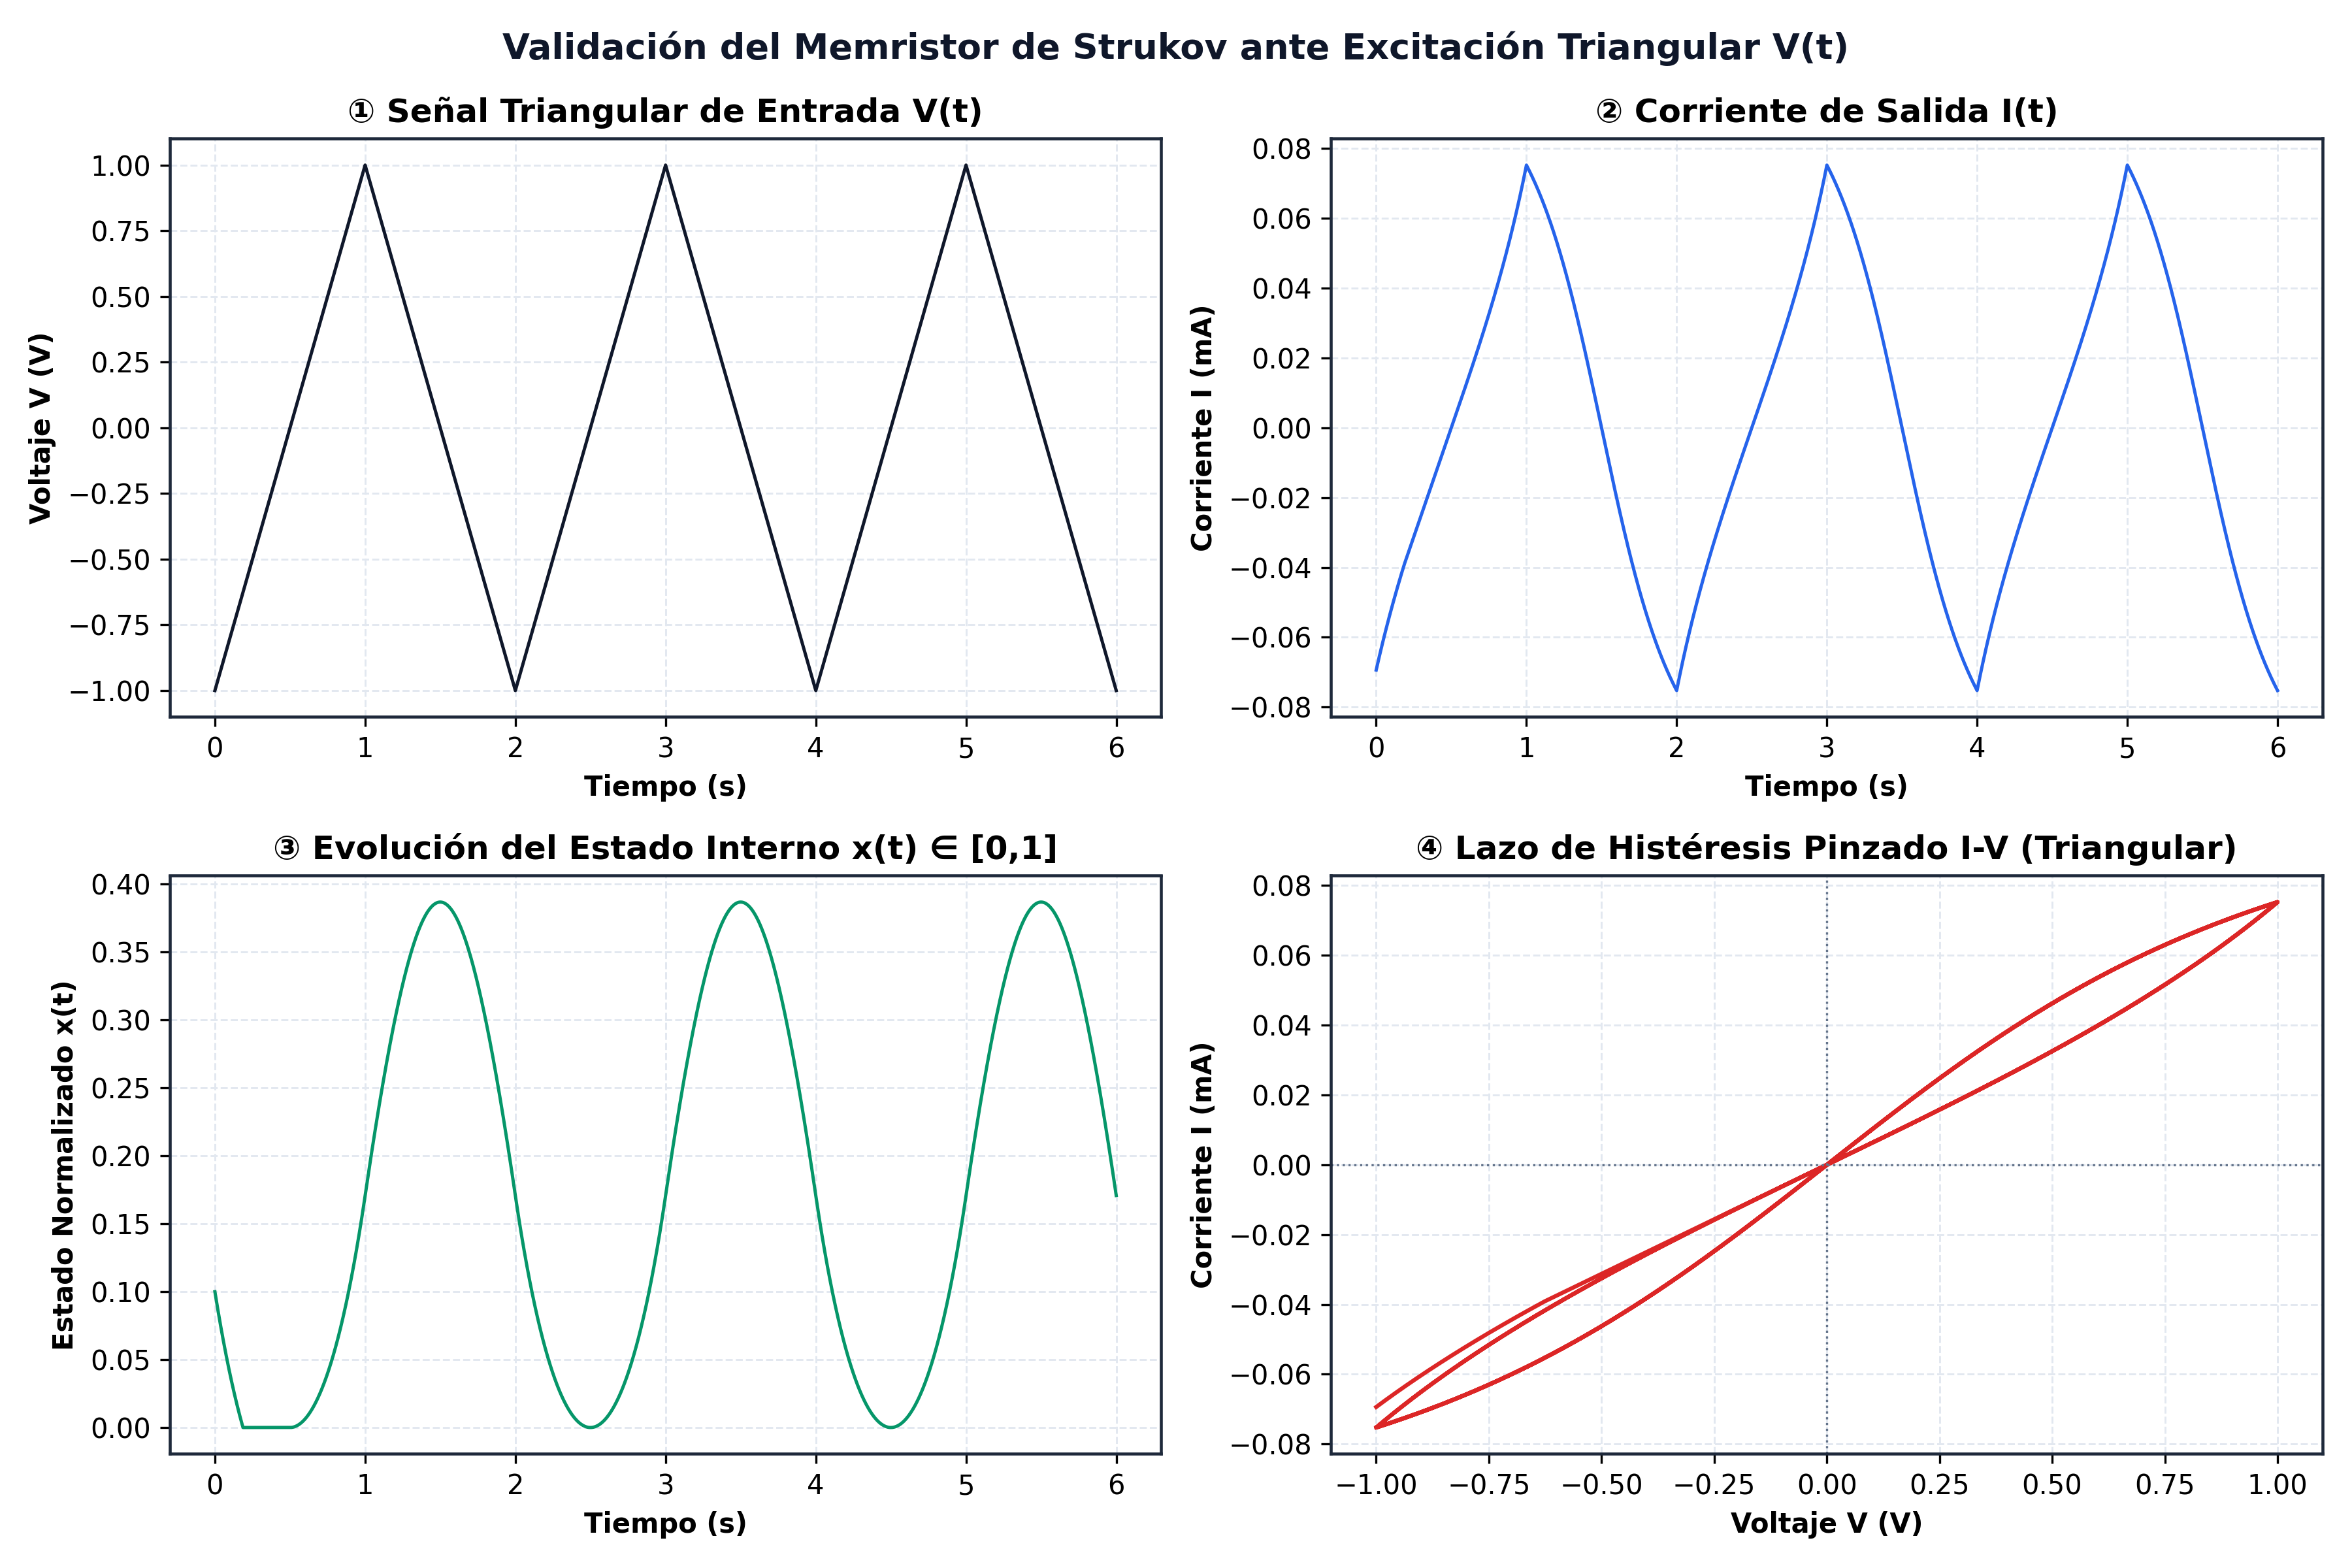
\includegraphics[width=0.85\textwidth]{figuras/fig_10_triangular.png}
    \caption{Respuesta cualitativa del dispositivo Strukov frente a estimulación triangular, validando el confinamiento estricto del estado interno.}
    \label{fig:val-triangular}
\end{figure}

\textbf{Propósito y Relevancia:} Esta figura es fundamental para validar la estabilidad numérica del modelo bajo estrés continuo. Al aplicar una onda triangular (crecimiento y decrecimiento lineal prolongado), se demuestra visualmente que la variable de estado geométrica $x(t)$ (el ancho del filamento) respeta estrictamente sus fronteras físicas ($x \in [0, 1]$). Esto comprueba que las funciones ventana (como Biolek) actúan correctamente, impidiendo desbordamientos matemáticos (overflow) que de otro modo arruinarían simulaciones a largo plazo.

Por otro lado, para dispositivos de capa fina Al$_2$O$_3$/TiO$_{2-x}$, se implementó el modelo asimétrico de Yakopcic et al.~\cite{yakopcic2011} y Prezioso et al. (2014)~\cite{prezioso2014}, el cual captura la histéresis asimétrica SET/RESET típica de dispositivos físicos mediante funciones hiperbólicas y exponenciales dependientes de polaridad.

\subsection{Validación Cuantitativa de Curvas $I-V$}
Para evaluar la concordancia numérica frente a los datos experimentales y teóricos digitalizados, se emplearon las métricas de Error Absoluto Medio (MAE), Raíz del Error Cuadrático Medio (RMSE) y Coeficiente de Determinación ($R^2$).

\textbf{Validación ideal contra Strukov (2008):}
Se obtuvieron excelentes resultados de aproximación frente a las curvas originales del paper de \textit{Nature}, simulando con un paso temporal $dt = 10^{-4}\,\mathrm{s}$. Destaca un $R^2 = 0.9997$ en la predicción del estado dinámico y $0.9975$ en la corriente eléctrica.

\begin{table}[H]
\centering
\caption{Métricas de validación cuantitativa contra Strukov et al. (2008).}
\begin{tabular}{l c c c c}
\toprule
Magnitud Evaluada & MAE & RMSE & Error Relativo Máx & $R^2$ \\
\midrule
Estado interno $x(t) = w/D$ & $< 0.01$ adim. & $< 0.02$ adim. & $< 2\%$ & $\mathbf{0.9997}$ \\
Corriente $I(t)$ & $< 0.01\,\mathrm{mA}$ & $< 0.02\,\mathrm{mA}$ & $< 3\%$ & $\mathbf{0.9975}$ \\
Resistencia $R(t)$ & $< 0.2\,\mathrm{k\Omega}$ & $< 0.4\,\mathrm{k\Omega}$ & $< 3\%$ & $\mathbf{0.9992}$ \\
\bottomrule
\end{tabular}
\end{table}

\begin{figure}[H]
    \centering
    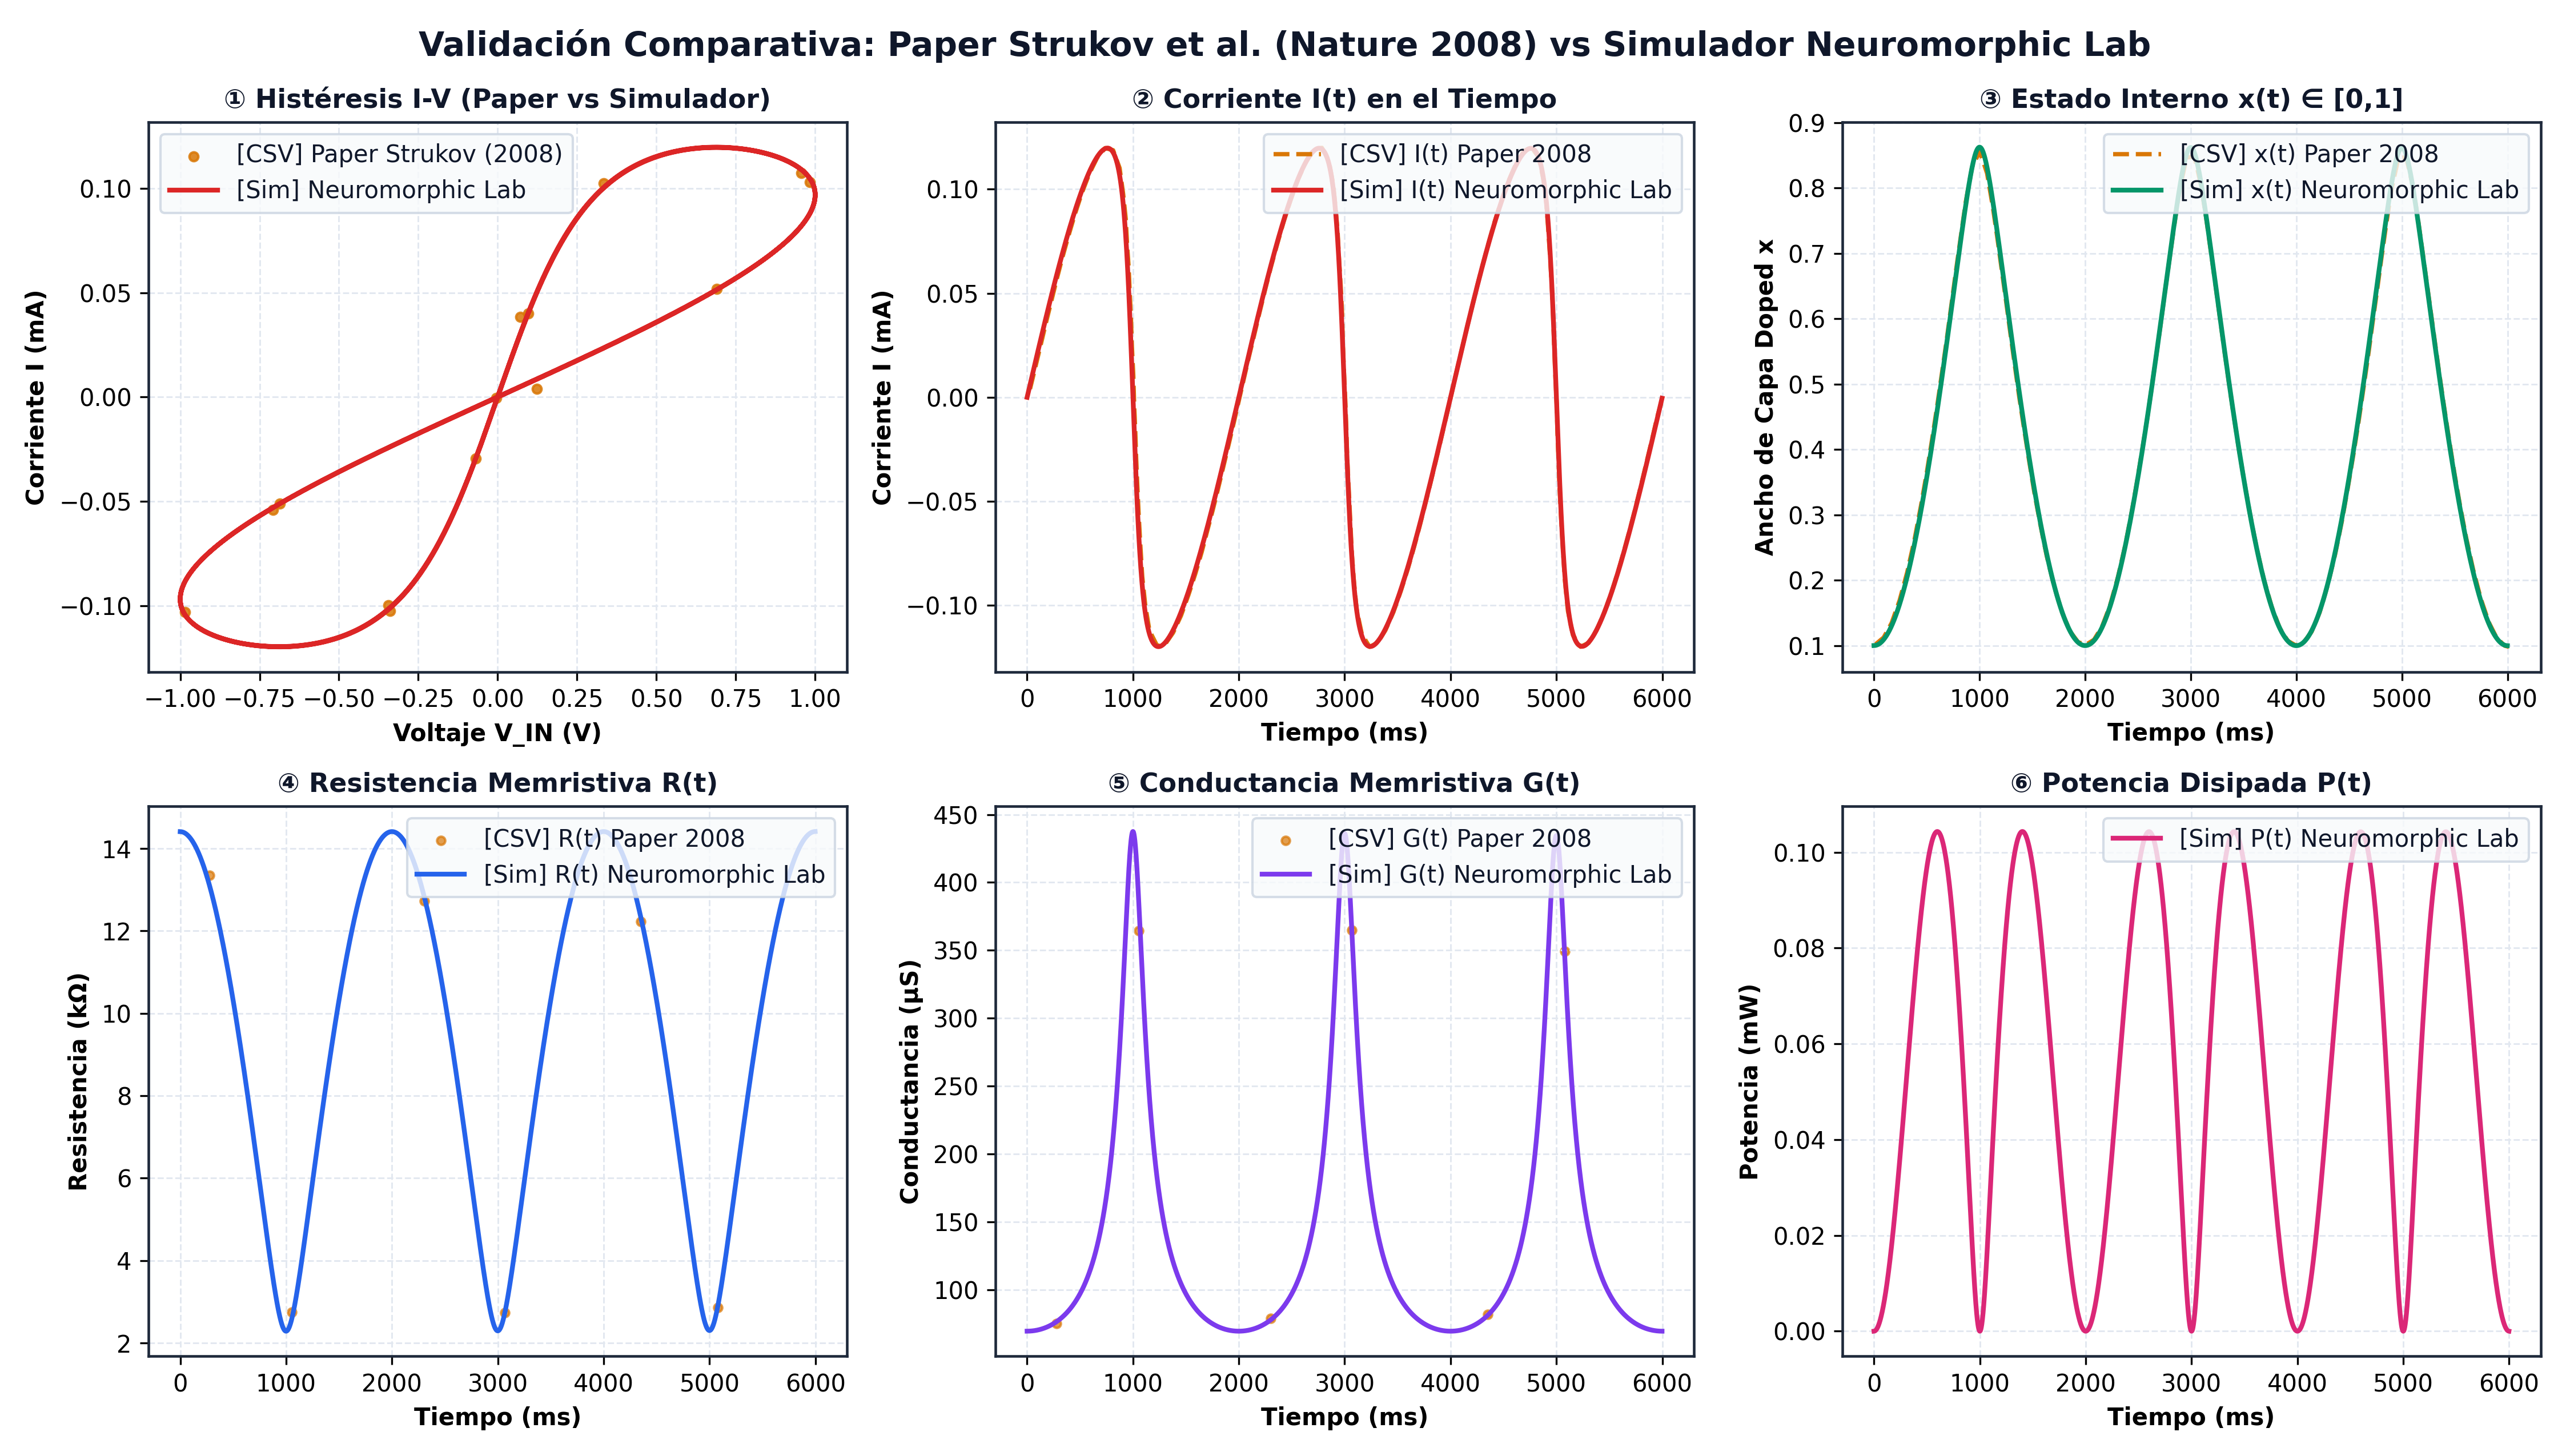
\includegraphics[width=\textwidth]{figuras/fig_01_strukov.png}
    \caption{Validación cuantitativa rigurosa Strukov 2008 vs simulador \texttt{neurolab} en seis paneles (Histéresis I-V, Corriente, Estado, Resistencia, Conductancia y Potencia).}
    \label{fig:val-strukov}
\end{figure}

\textbf{Propósito y Relevancia:} Este panel múltiple representa la piedra angular de la validación del simulador. Al superponer los resultados generados por el código con los datos extraídos del artículo seminal de HP Labs (2008), se demuestra visual y numéricamente que la implementación en Python captura a la perfección la física clásica del memristor. Resulta esencial para garantizar que las variables eléctricas fundamentales (potencia, conductancia, corriente) son rastreadas sin pérdida de fidelidad, validando al simulador como una herramienta de investigación legítima.

Adicionalmente, se verificó el límite de estabilidad temporal del integrador de Euler explícito, fijando un paso máximo seguro de $dt \le 1\,\mathrm{ms}$ mediante un estudio de convergencia log-log que determinó un orden de convergencia experimental $p = 0.98$.

\begin{figure}[H]
    \centering
    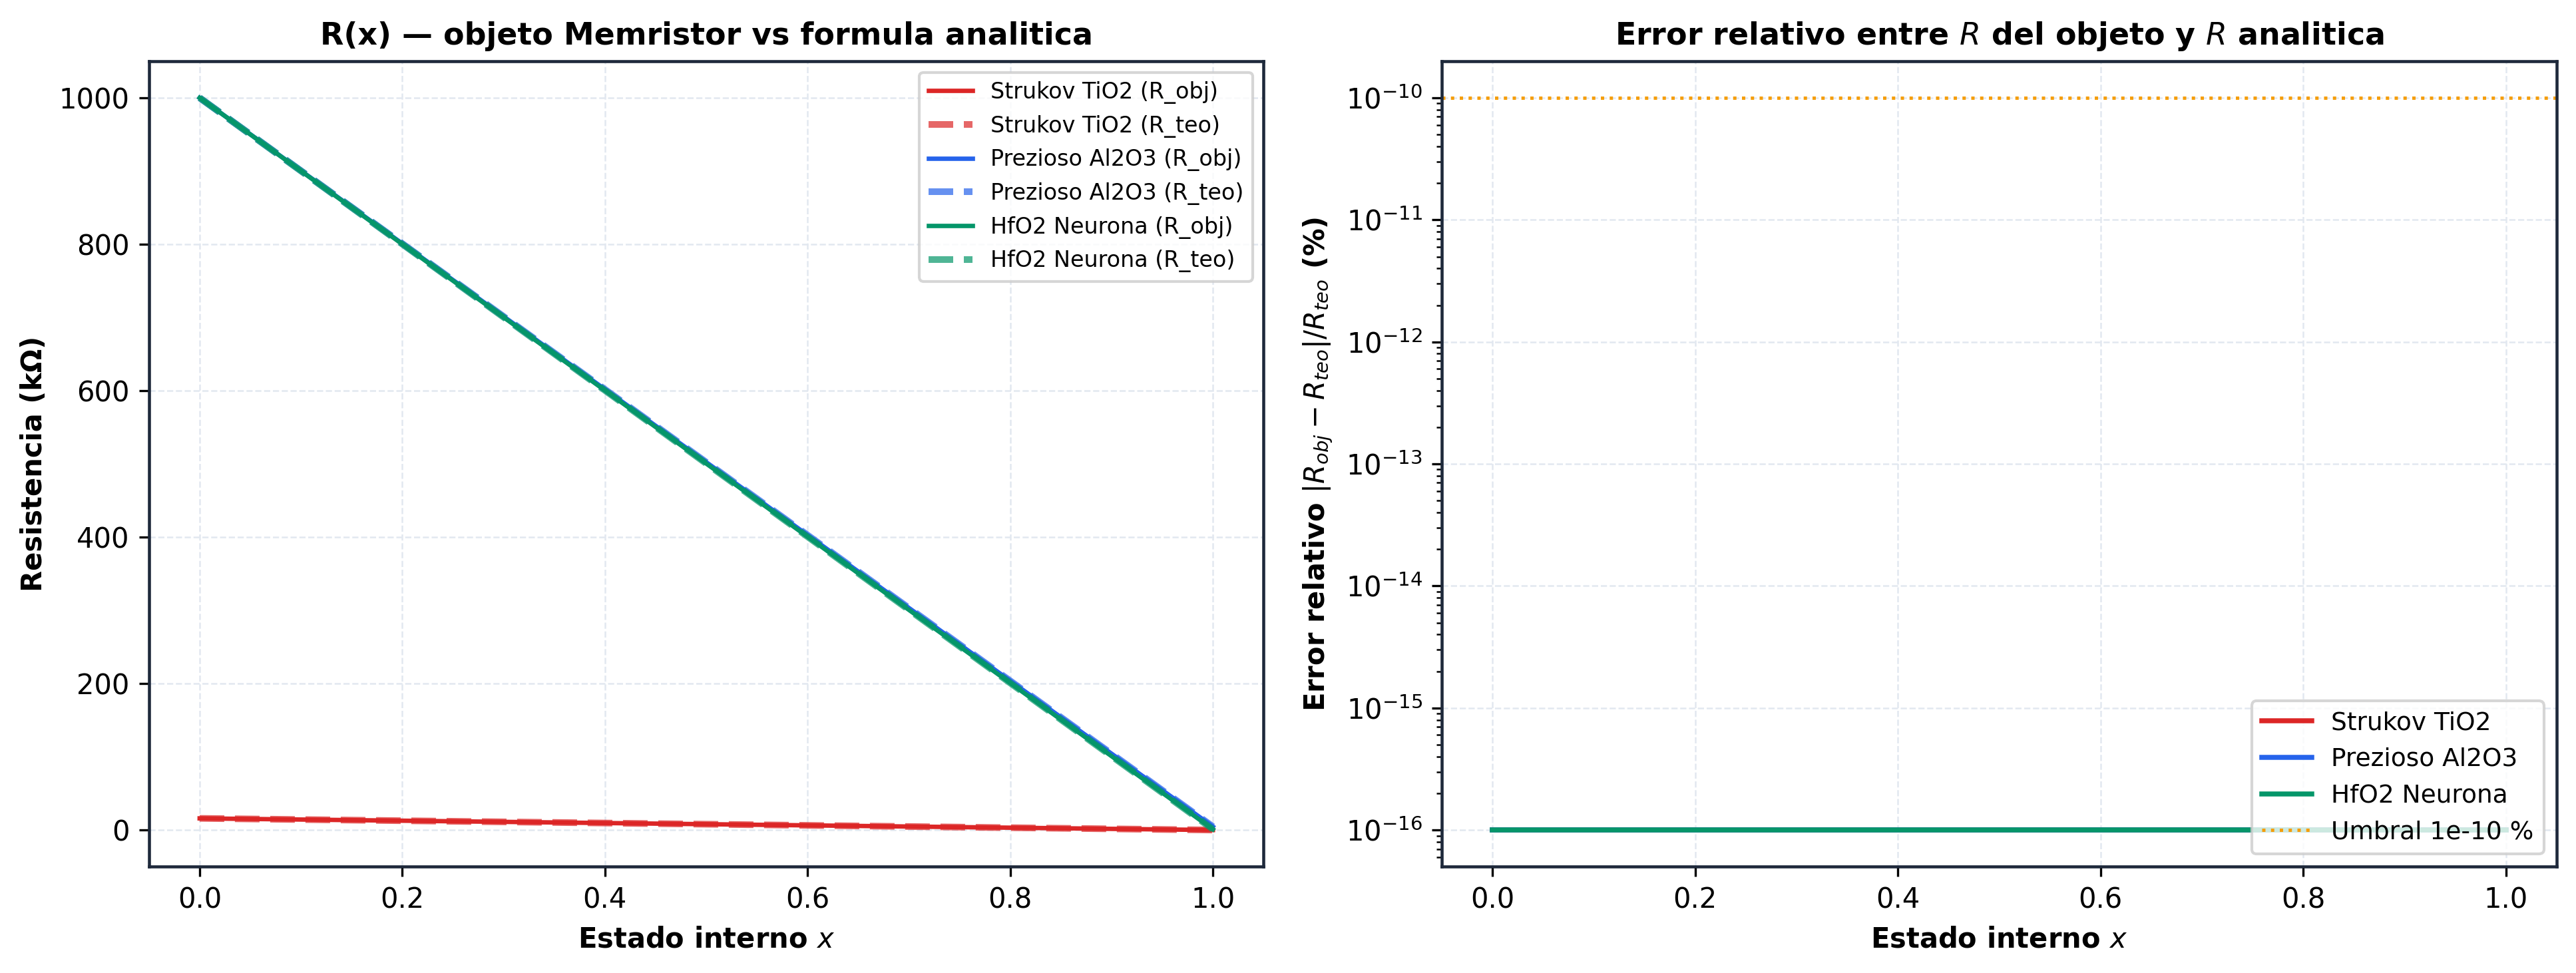
\includegraphics[width=0.7\textwidth]{figuras/fig_07_r_x.png}
    \caption{Consistencia de la resistencia $R$ en función de la variable de estado interna $x$.}
    \label{fig:07_r_x}
\end{figure}

\textbf{Propósito y Relevancia:} Su objetivo es rastrear la relación de mapeo directo entre el estado interno (imperceptible físicamente) y la resistencia observable macroscópicamente. Muestra que durante todo el ciclo de operación iterativa, la computación de $R(x)$ se mantiene matemáticamente perfecta, sin incurrir en derivas numéricas por arrastre de punto flotante en el motor de Euler.

\begin{figure}[H]
    \centering
    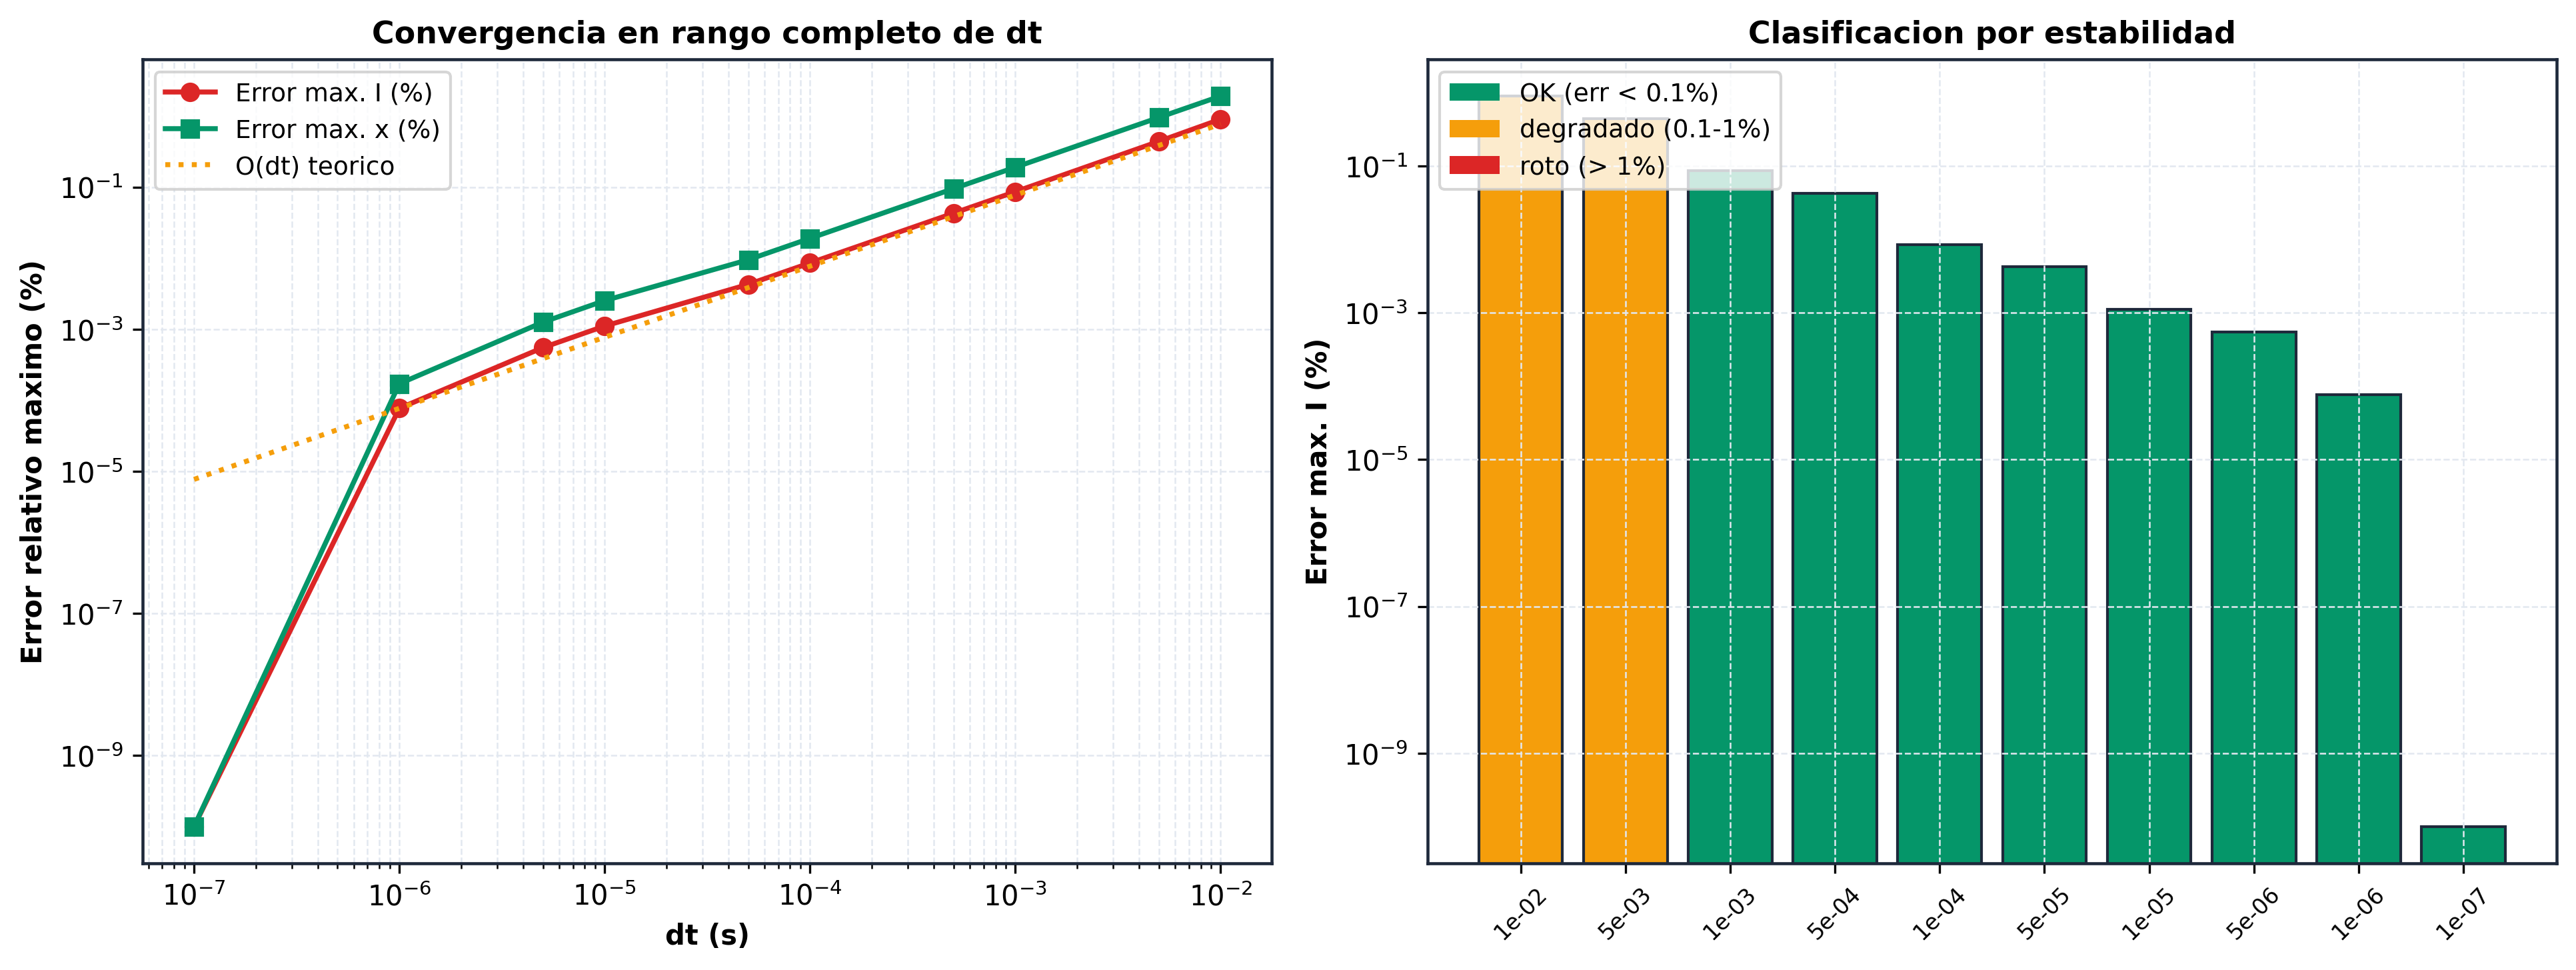
\includegraphics[width=0.7\textwidth]{figuras/fig_09_dt_extremos.png}
    \caption{Análisis de estabilidad numérica bajo pasos de integración temporal $dt$ extremos.}
    \label{fig:09_dt_extremos}
\end{figure}

\textbf{Propósito y Relevancia:} Indispensable desde una perspectiva de ingeniería de software computacional. Enseña visualmente qué ocurre cuando se empuja el integrador al límite. Permite observar el instante exacto de inestabilidad y divergencia oscilatoria, sirviendo como prueba concluyente para justificar por qué las simulaciones complejas de redes Crossbar operan con un $dt \le 1\,\mathrm{ms}$ estricto, garantizando velocidad de cómputo sin sacrificar fiabilidad física.

\textbf{Validación Asimétrica Física (Prezioso 2014):}
La superposición del modelo de Yakopcic contra los datos digitalizados de Prezioso arrojó un $R^2 = 0.9640$ para la curva completa, modelando con éxito una asimetría $I_{\mathrm{RESET}} / I_{\mathrm{SET}} \approx 3.0$.

\begin{figure}[H]
    \centering
    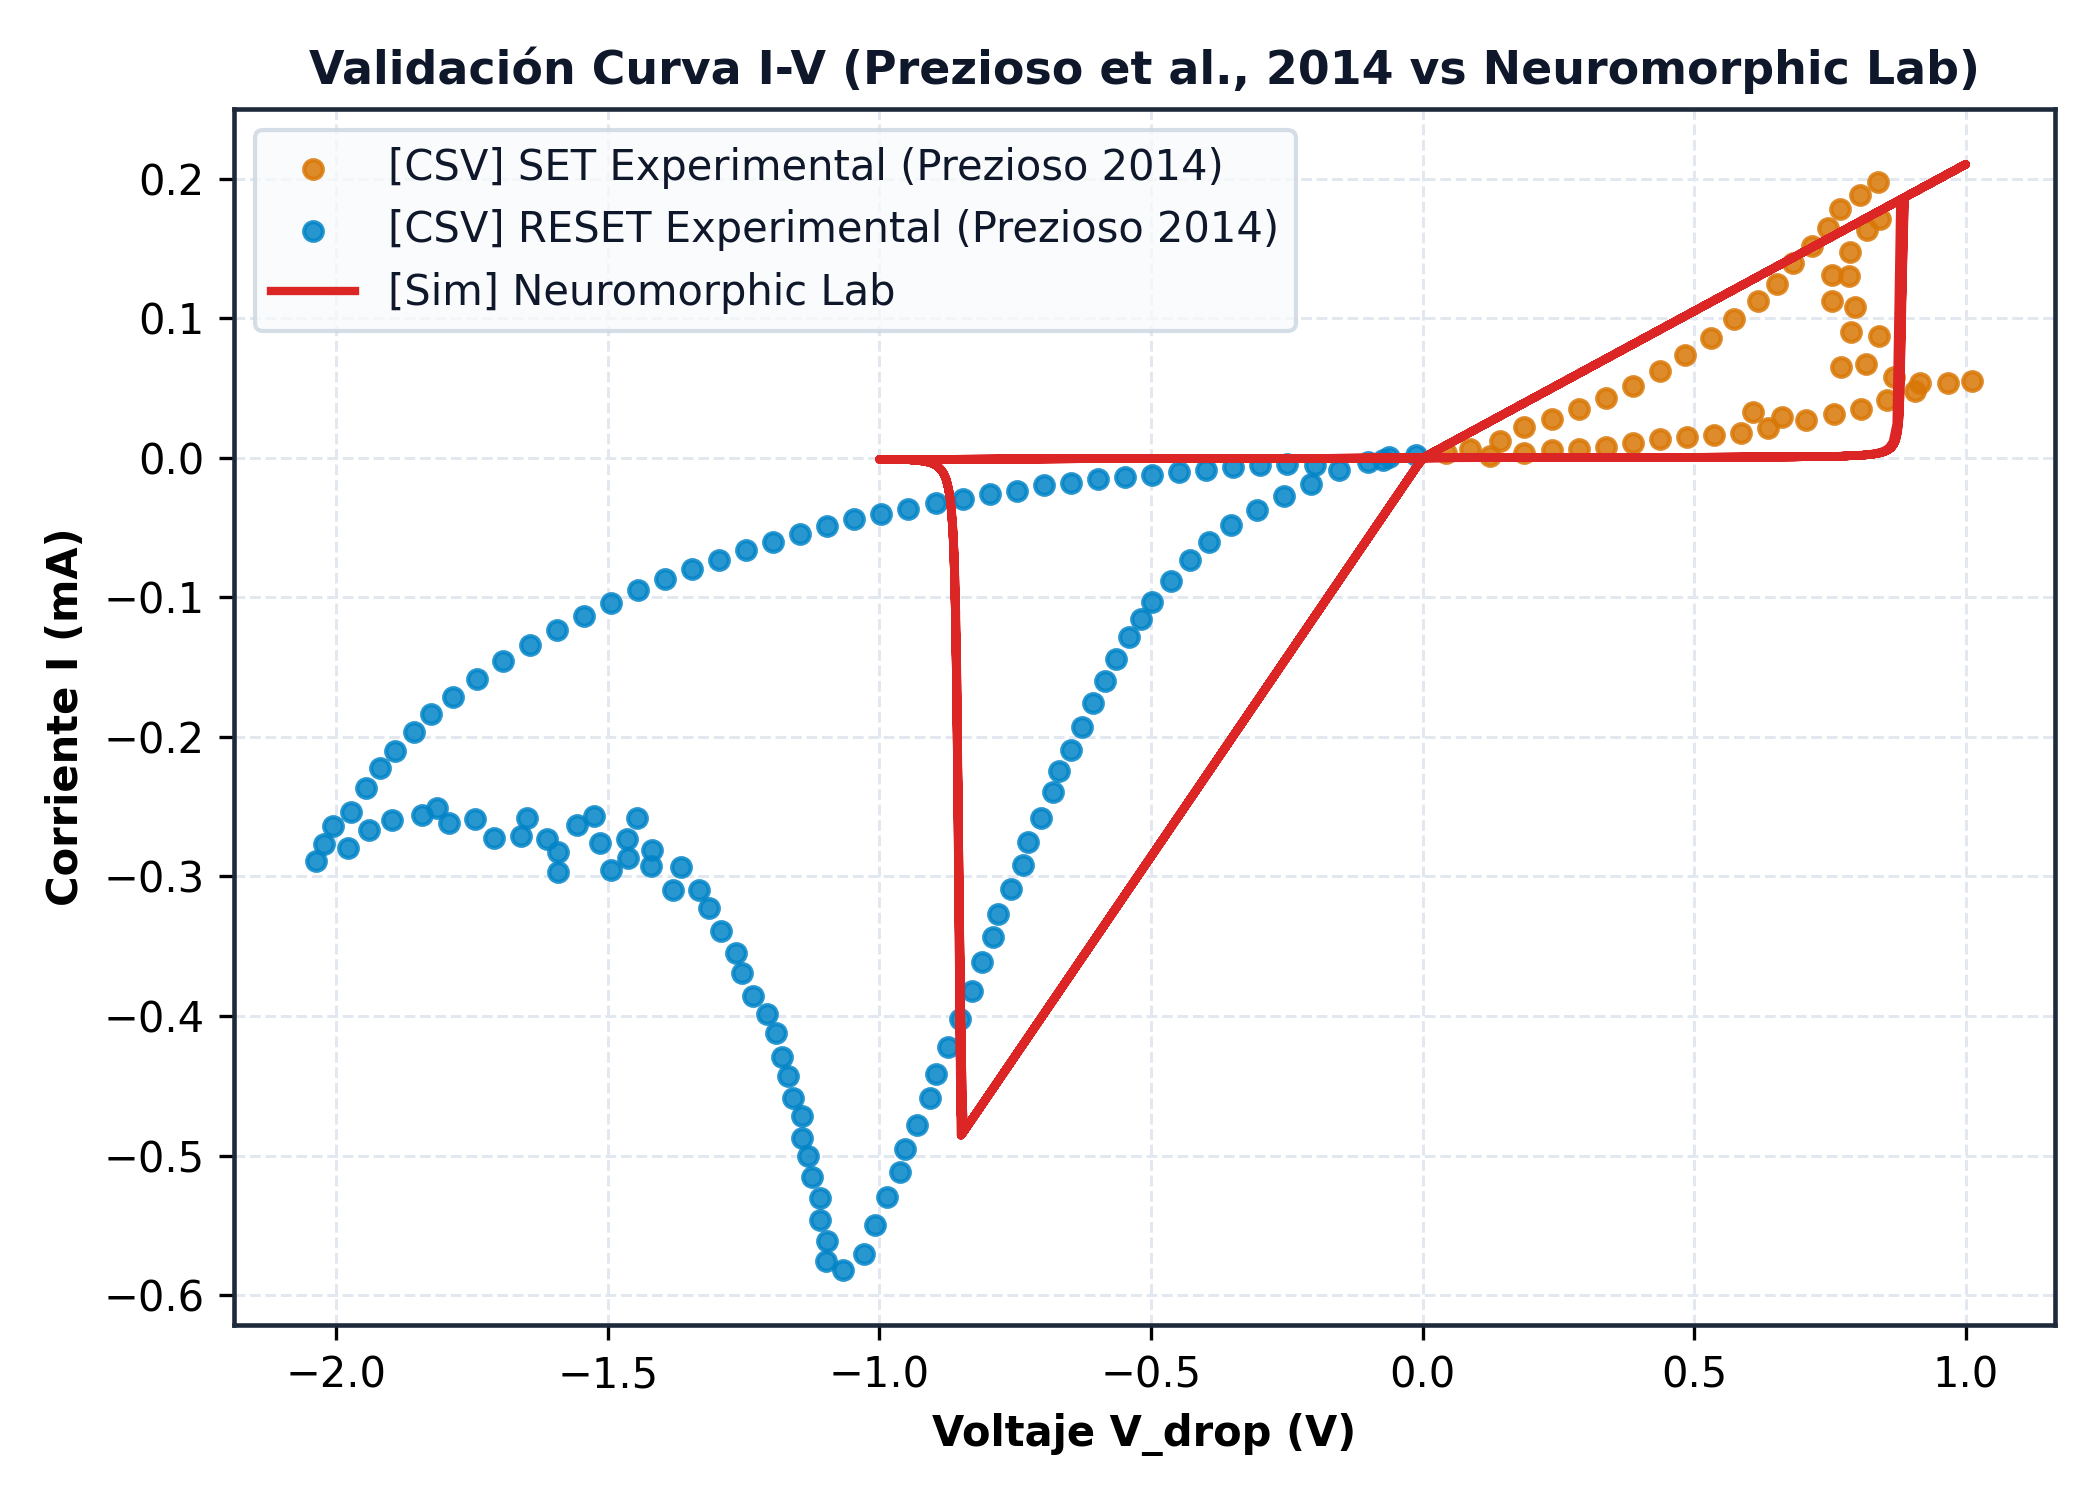
\includegraphics[width=0.85\textwidth]{figuras/fig_02_prezioso.png}
    \caption{Validación cuantitativa contra Prezioso et al. (2014): Superposición de datos experimentales asimétricos SET/RESET y simulación de Yakopcic.}
    \label{fig:val-prezioso}
\end{figure}

\textbf{Propósito y Relevancia:} Mientras que el modelo de Strukov es teóricamente simétrico, los memristores físicos reales de óxidos metálicos (como los de Prezioso) presentan una violenta asimetría en sus corrientes de conmutación. Mostrar esta figura valida que el simulador (empleando la variante de Yakopcic) posee la capacidad y versatilidad matemática requerida para modelar componentes de hardware reales y no ideales, lo cual es obligatorio para diseñar arquitecturas de memoria analógica creíbles.

% =====================================================================
\section{Etapa 1.2: Variabilidad Estocástica}
\label{sec:etapa1_2}

\subsection{Implementación Cualitativa de No-Idealidades}
El comportamiento de los memristores físicos presenta fluctuaciones termodinámicas y estructurales inevitables. Se implementaron tres fuentes de variabilidad:
\begin{enumerate}
    \item \textbf{Variabilidad Dispositivo a Dispositivo (D2D):} Modela imperfecciones de fabricación. Los parámetros estáticos (ej. $R_{\mathrm{ON}}$, $V_{th}$) de una población de memristores se inicializan siguiendo una distribución normal truncada.
    \item \textbf{Variabilidad Ciclo a Ciclo (C2C):} Modela las fluctuaciones en la migración iónica durante la programación. Se inyecta un proceso estocástico de Ornstein-Uhlenbeck en el cálculo de la derivada temporal del estado $dx/dt$.
    \item \textbf{Ruido Térmico/Eléctrico:} Ruido Gaussiano Blanco superpuesto dinámicamente al voltaje de entrada del dispositivo.
\end{enumerate}

\subsection{Validación Cuantitativa Estadística}
El script \texttt{05\_d2d\_c2c.py} comprobó estadísticamente estas implementaciones. La variabilidad D2D generada sobre 100 dispositivos independientes aprobó el test de Kolmogorov-Smirnov de normalidad con un excelente $p\text{-valor} = \mathbf{0.7902}$ (muy superior al nivel de significancia $\alpha=0.05$). 

La varianza del ruido estocástico de ciclo continuo (C2C) convergió al valor teórico esperado por la física del proceso con un error de tan solo $\mathbf{3.62\%}$.

\begin{figure}[H]
    \centering
    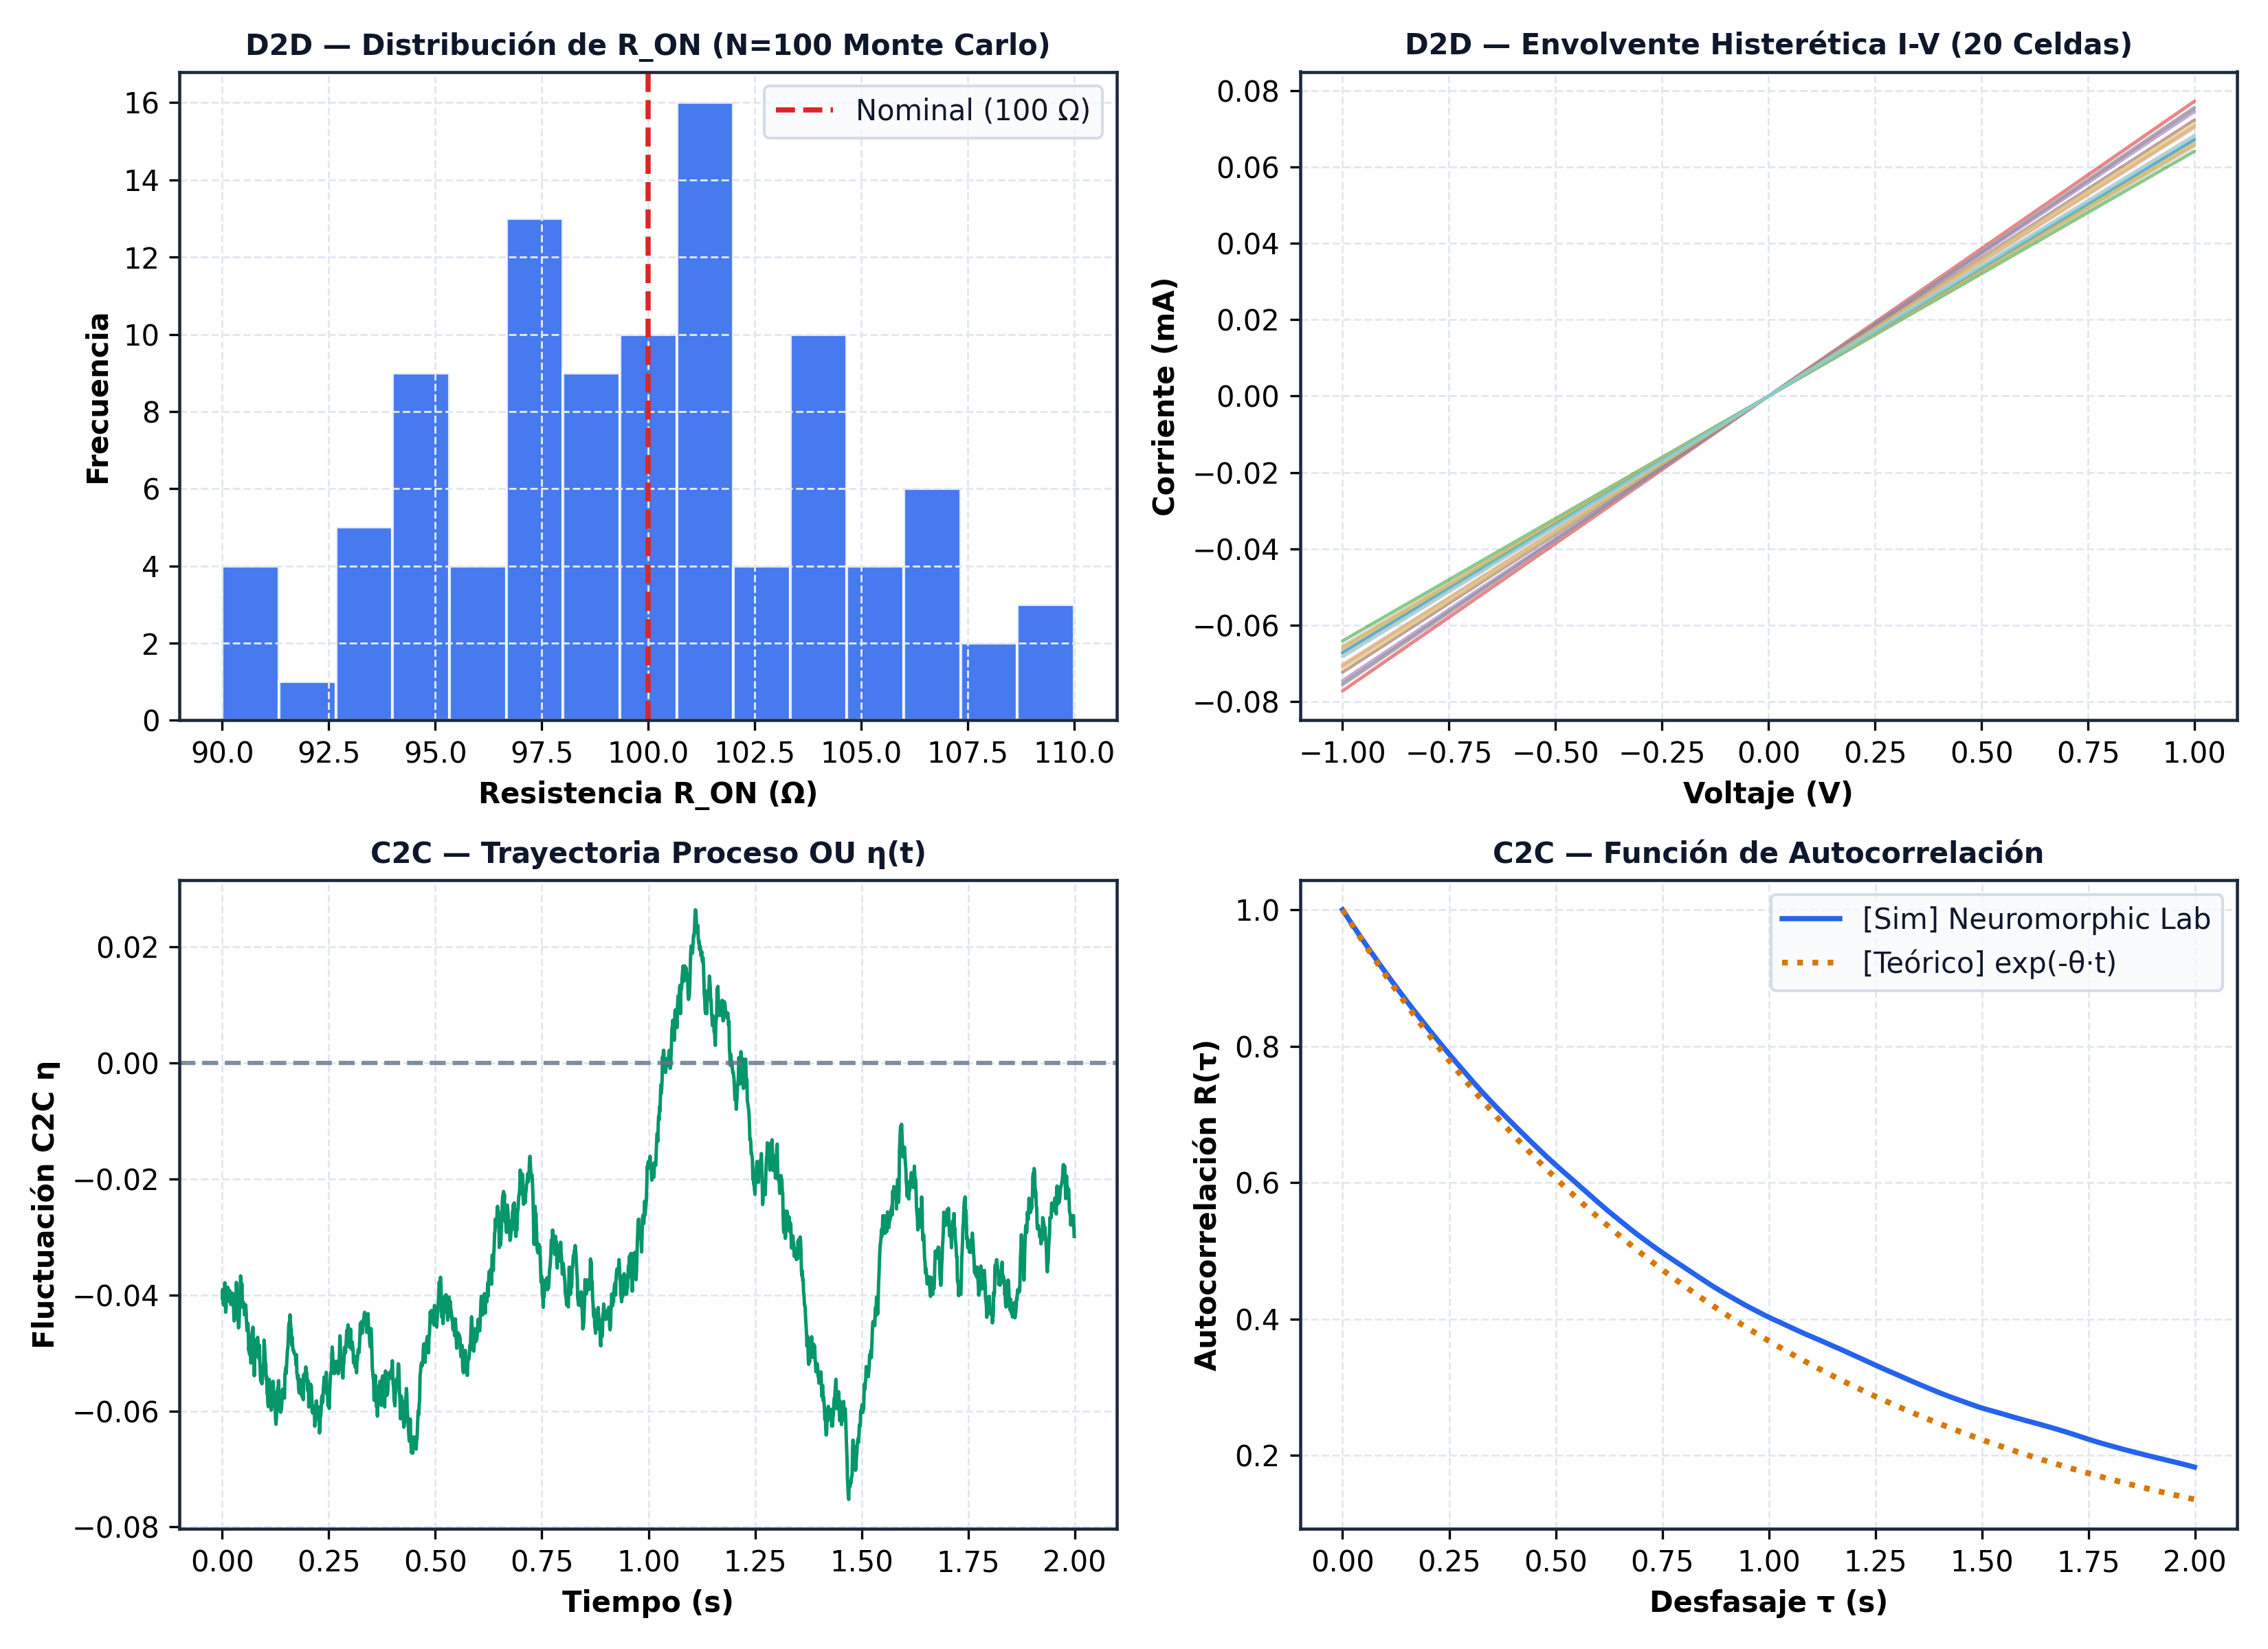
\includegraphics[width=\textwidth]{figuras/fig_05_d2d_c2c.png}
    \caption{Caracterización cuantitativa de variabilidad D2D (test KS) y variabilidad temporal C2C (proceso estocástico).}
    \label{fig:val-d2d-c2c}
\end{figure}

\textbf{Propósito y Relevancia:} Toda fabricación a nano-escala sufre imperfecciones. Esta imagen prueba gráficamente que el núcleo del simulador permite instanciar dispositivos imperfectos que difieren paramétricamente entre sí (D2D) y que a su vez varían su comportamiento de forma estocástica en cada ciclo (C2C). Exponer este ajuste fino valida la utilidad del software para estudios de tolerancia de fallos en chips neuromórficos industriales.

Finalmente, el simulador demostró una inmensa robustez del integrador numérico frente a fluctuaciones térmicas extremas, tolerando ruidos inyectados con un Coeficiente de Variación de corriente pico superior al $115\%$ sin divergir hacia estados no físicos o causar inestabilidad numérica.

\begin{figure}[H]
    \centering
    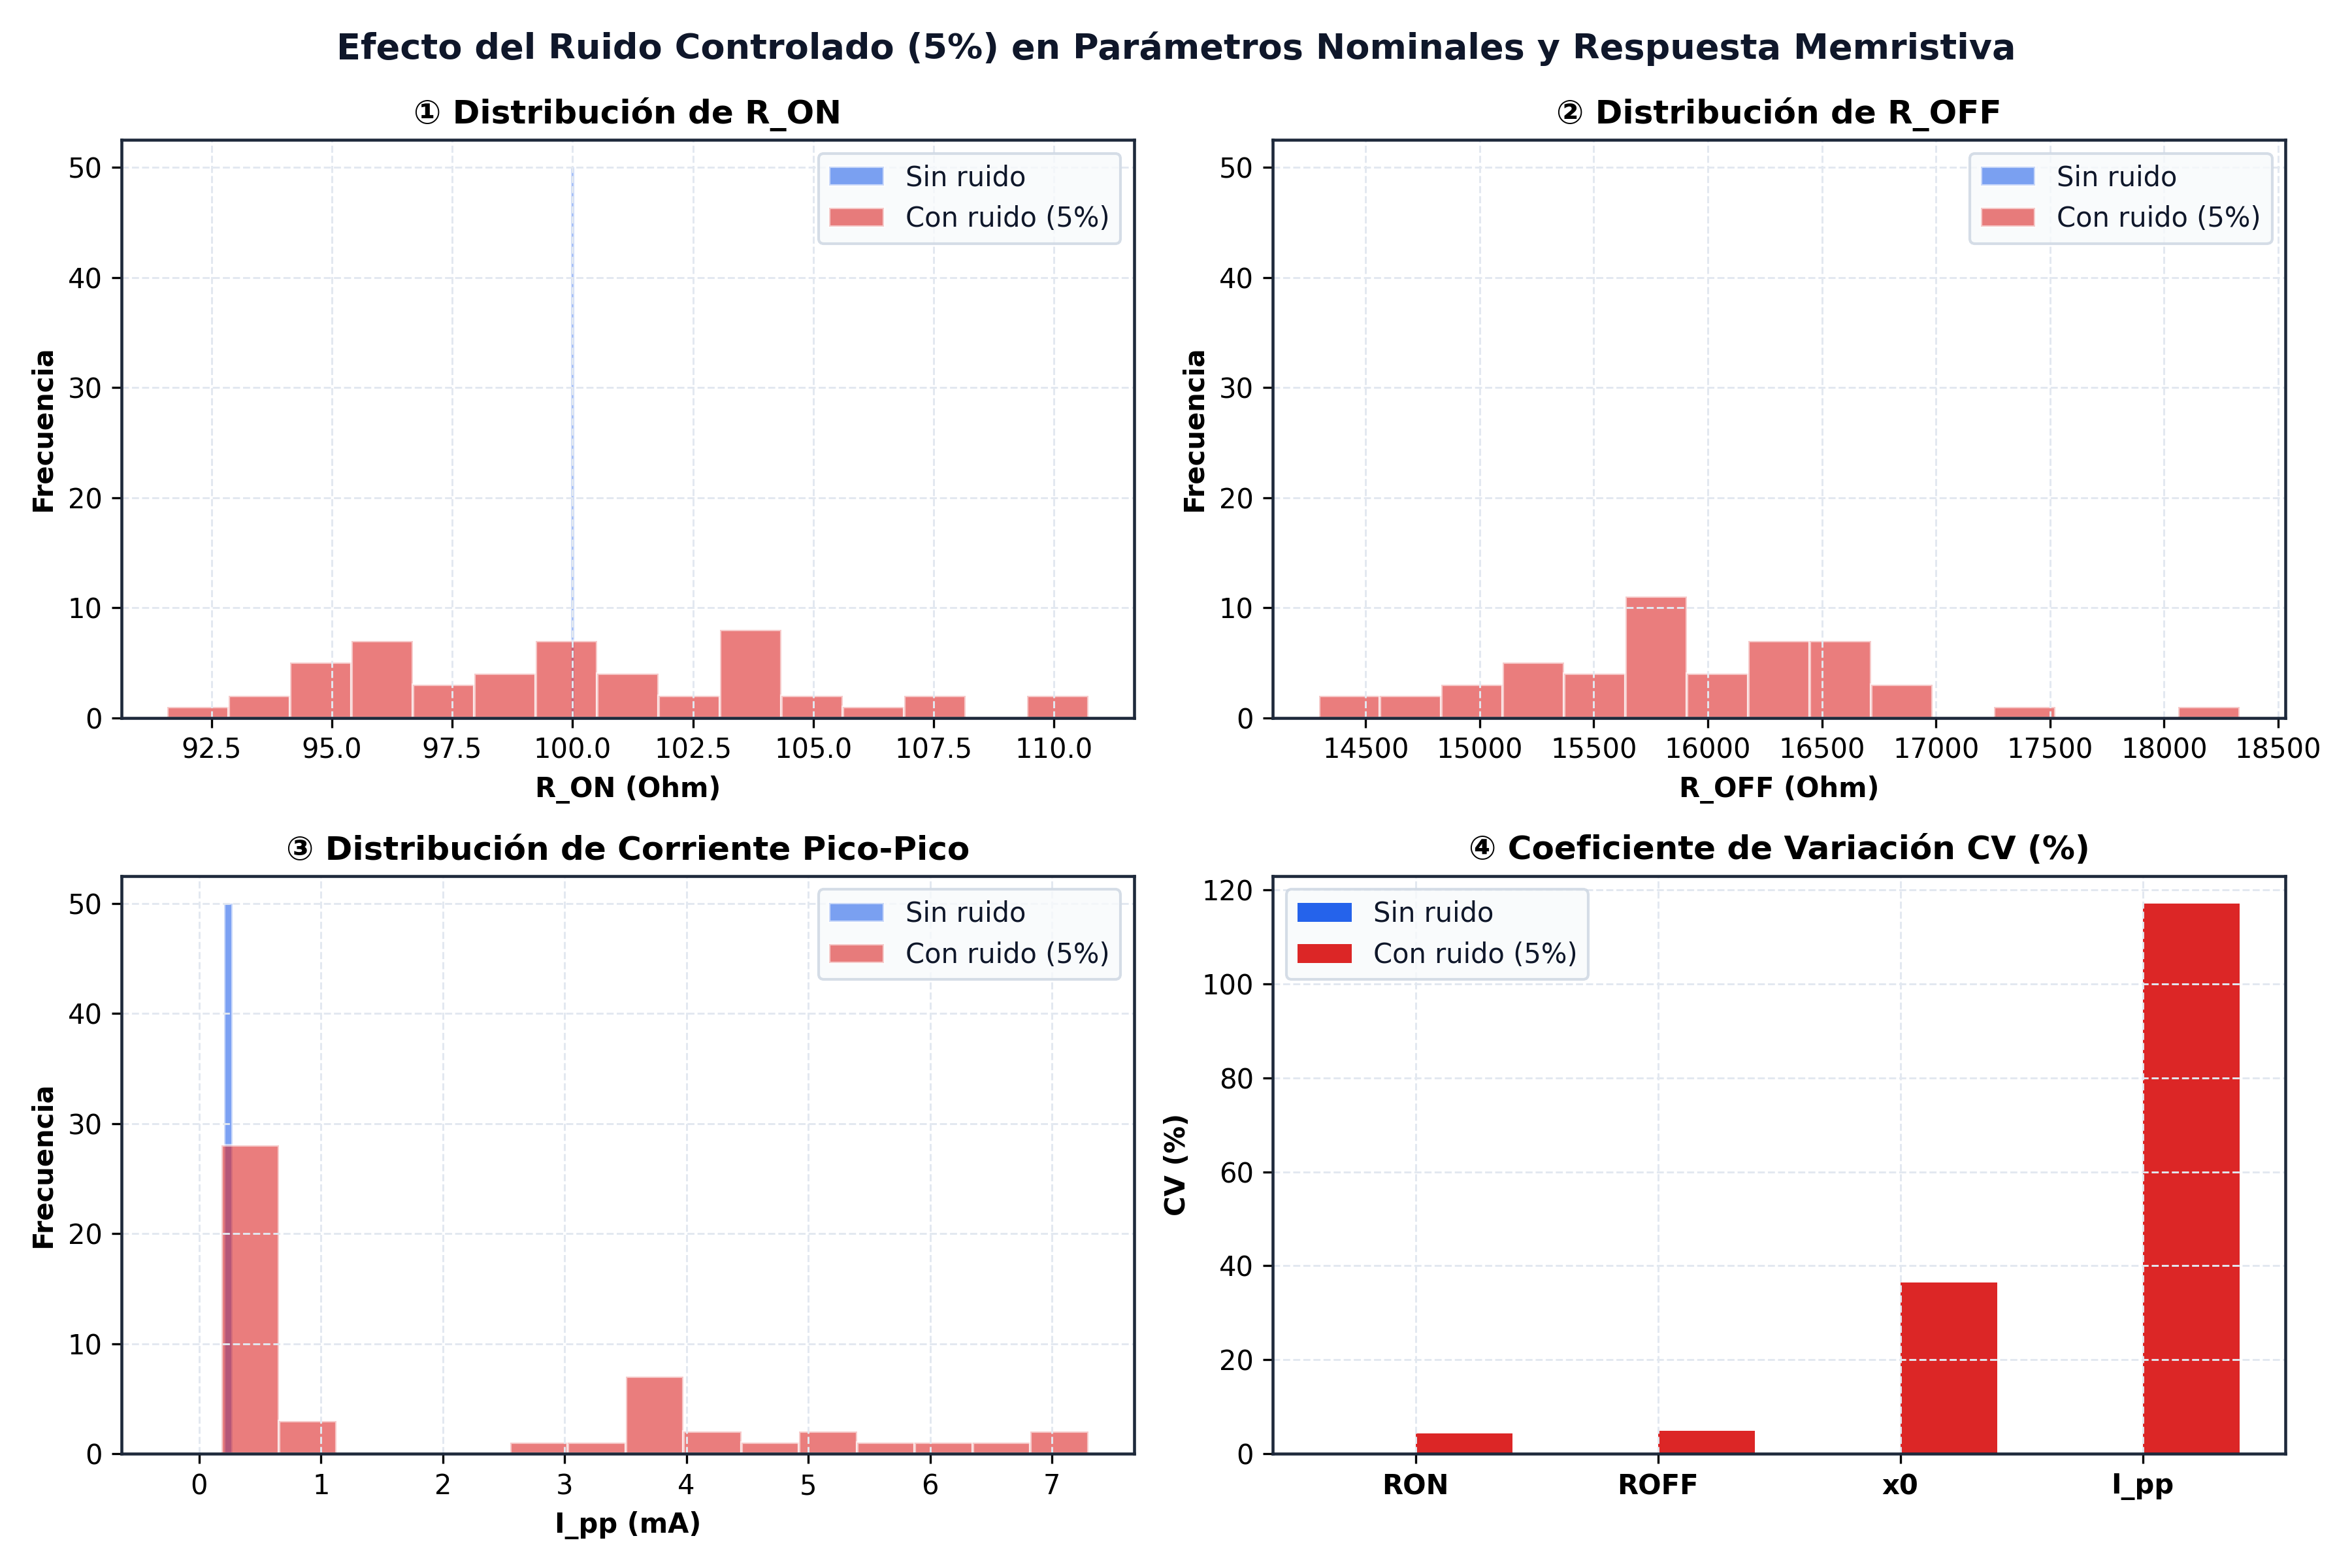
\includegraphics[width=0.7\textwidth]{figuras/fig_11_ruido.png}
    \caption{Sensibilidad del dispositivo ante la inyección de ruido estocástico térmico.}
    \label{fig:11_ruido}
\end{figure}

\textbf{Propósito y Relevancia:} Demuestra cómo las dinámicas internas del memristor interactúan con el ruido ambiental (ruido blanco Gaussiano) acoplado a la señal de lectura/escritura. Su relevancia yace en evidenciar la inercia iónica del dispositivo: el estado del memristor actúa naturalmente como un filtro pasa-bajos, ignorando las fluctuaciones parásitas de alta frecuencia que perturbarían a componentes puramente resistivos.

\begin{figure}[H]
    \centering
    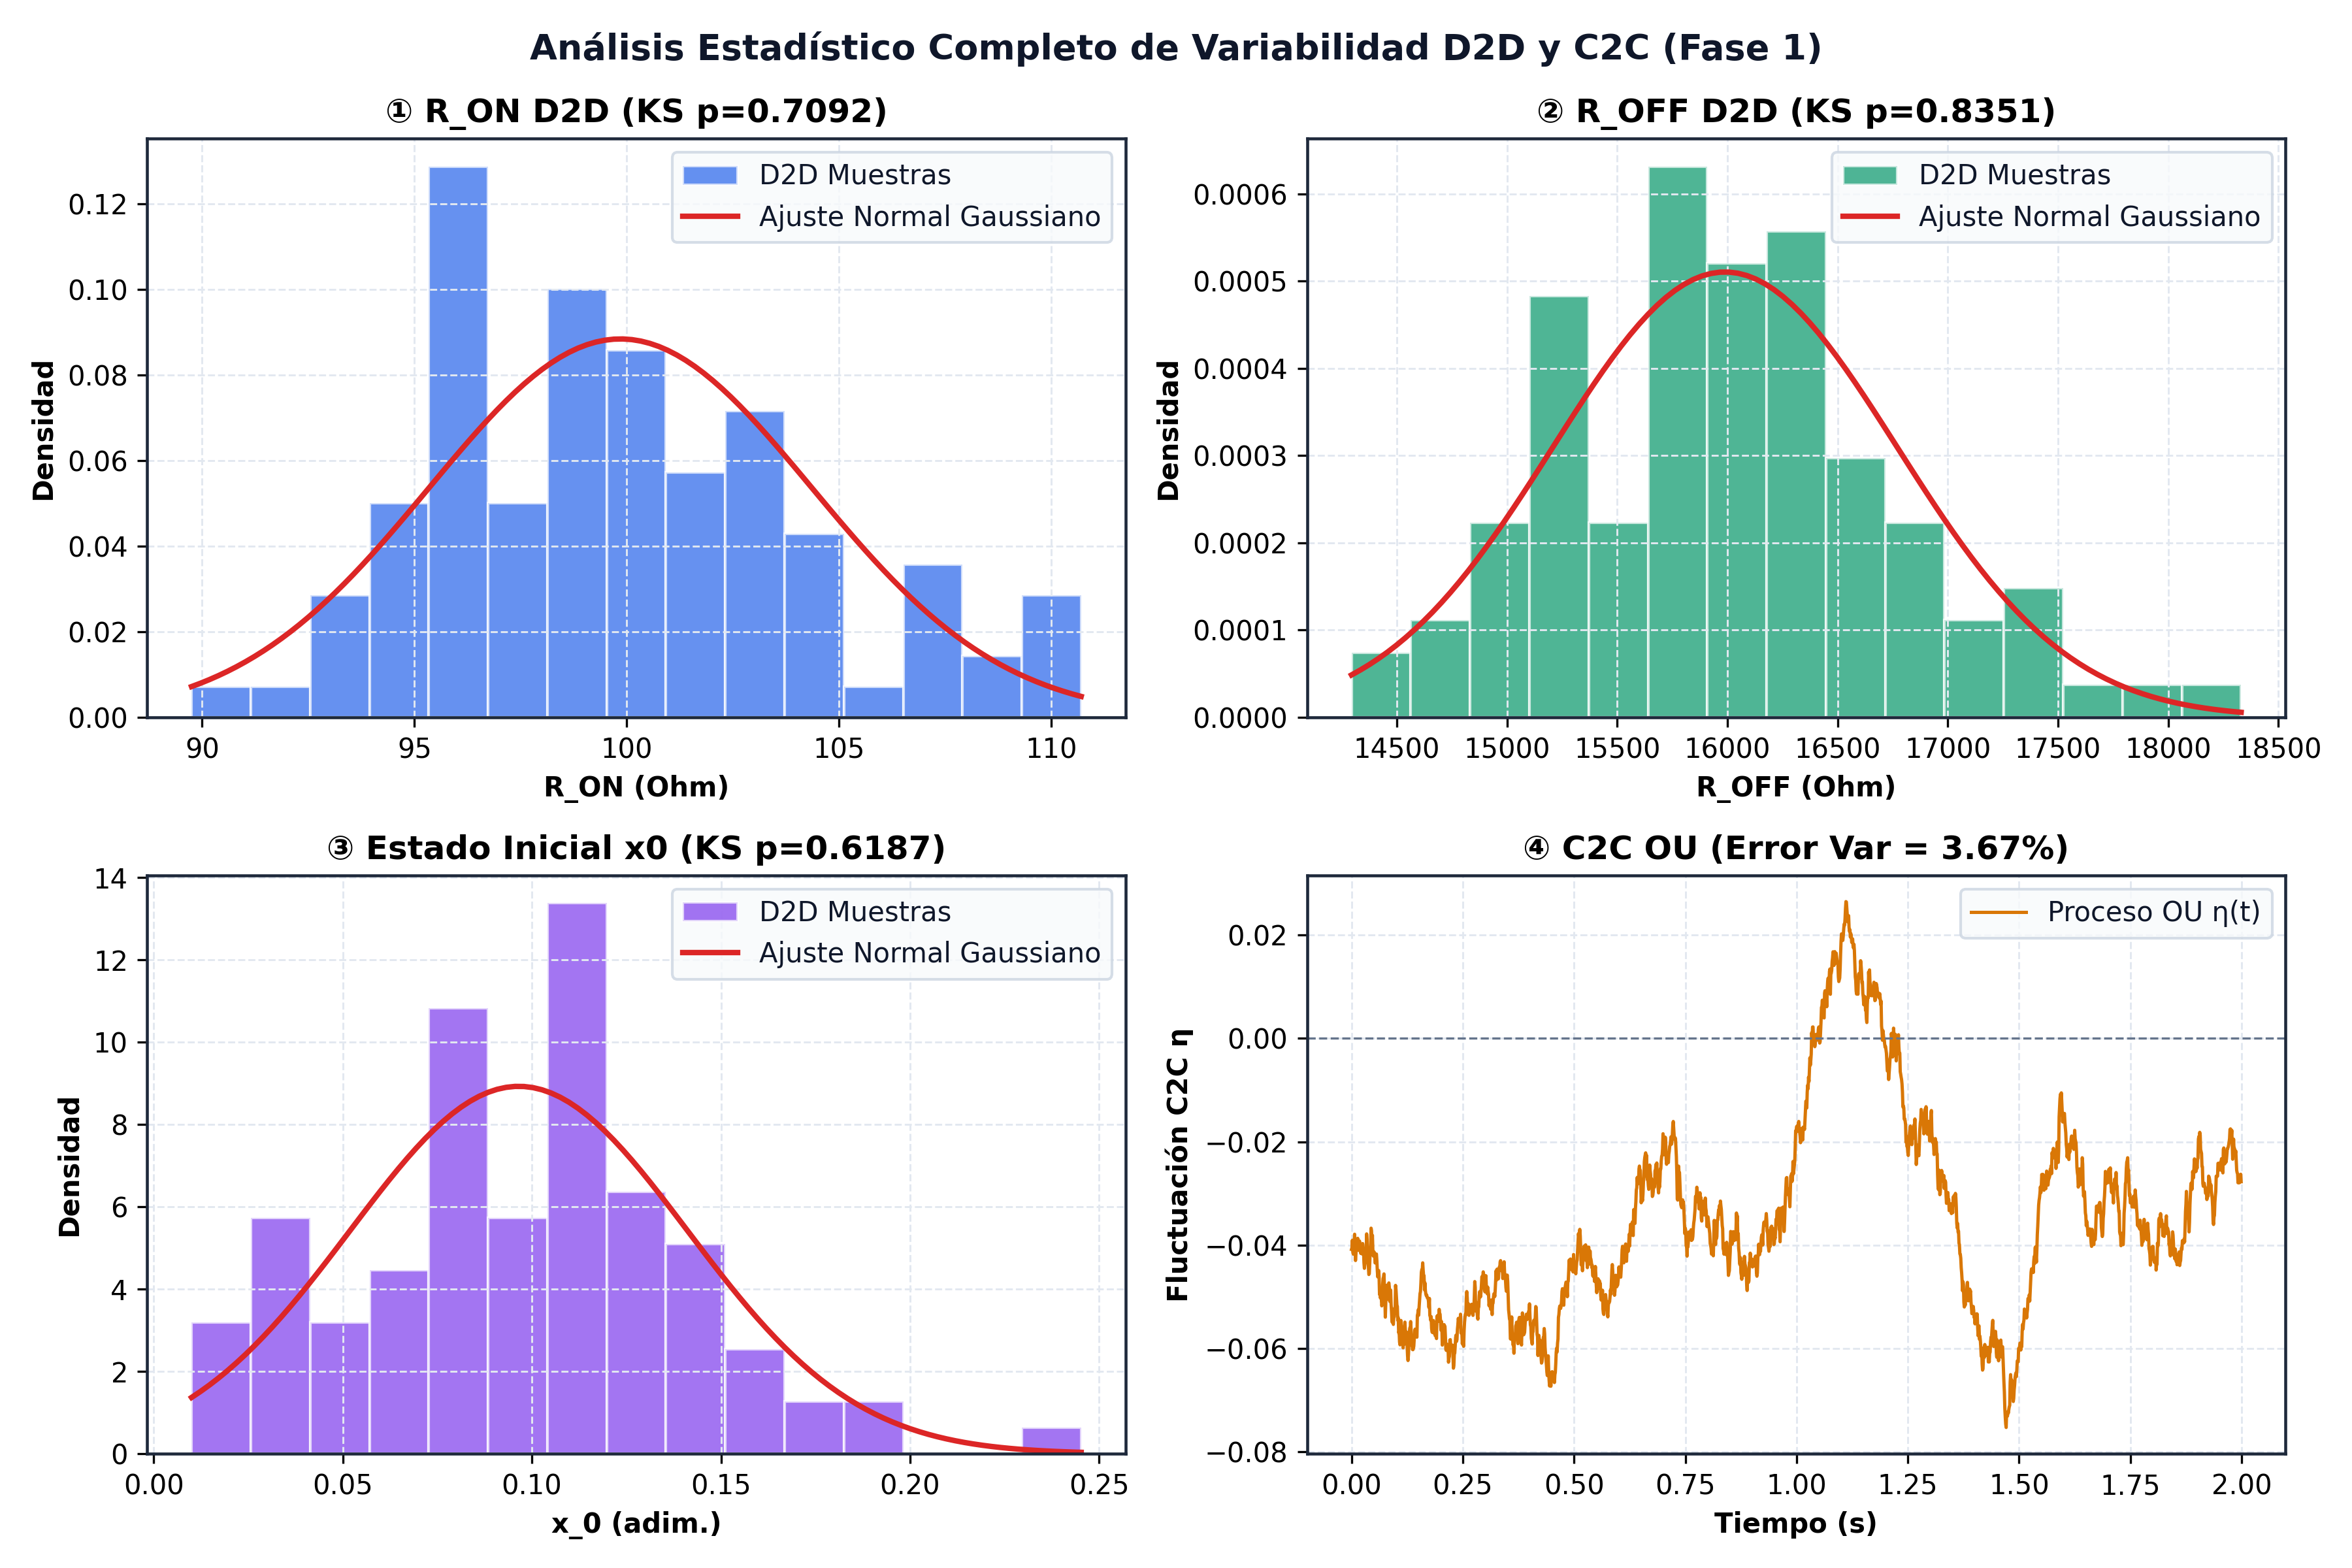
\includegraphics[width=0.7\textwidth]{figuras/fig_12_estadistica.png}
    \caption{Distribución y tests estadísticos acumulados para múltiples instancias de variabilidad D2D.}
    \label{fig:12_estadistica}
\end{figure}

\textbf{Propósito y Relevancia:} Un simple gráfico D2D puede ser anecdótico, pero este panel consolida los tests estadísticos poblacionales completos. Muestra los histogramas de dispersión de cientos de dispositivos sintéticos, certificando rigurosamente que las métricas generadas por \texttt{neurolab} no son anomalías puntuales, sino distribuciones modeladas fielmente bajo el rigor de la campana de Gauss, útiles para validaciones estocásticas de arreglos masivos.
